\documentclass[10pt]{article}

\usepackage[a4paper,margin=0.58in]{geometry}
\usepackage{amsmath}
\usepackage{graphicx}
\usepackage{url}
\usepackage{multicol}

\graphicspath{{figures/}}
\setlength{\parskip}{3pt}
\setlength{\parindent}{1em}
\setlength{\textfloatsep}{4pt plus 1pt minus 1pt}
\setlength{\intextsep}{4pt plus 1pt minus 1pt}
\setlength{\floatsep}{4pt plus 1pt minus 1pt}

\makeatletter
\renewcommand\section{\@startsection{section}{1}{\z@}%
  {1.5ex plus .4ex minus .2ex}{.5ex plus .1ex}%
  {\normalfont\large\bfseries}}
\makeatother

\newcommand{\SNR}{\mathrm{SNR}}
\newcommand{\SNReff}{\mathrm{SNR}_{\mathrm{eff}}}
\newcommand{\CRB}{\mathrm{CRB}}

\title{\vspace{-1.2em}\bfseries Broadband Transient Localization over WDM Fibre:\\
Empirical Fusion Guided by Pairwise Bounds}
\author{Rafael Vieira$^{(1)}$, Pedro Freire$^{(1)}$, Sergei Turitsyn$^{(1)}$\\[3pt]
\small (1) Aston University, United Kingdom\\
\small \texttt{randr24@aston.ac.uk}}
\date{}

\begin{document}
\maketitle
\vspace{-2.1em}

\begin{abstract}
Transient localization from wavelength-dependent polarization signatures in WDM fibres. Chromatic dispersion maps distance to inter-channel delay. At 5-km RMSE, dispersion-aware fusion cuts SNR by 30 dB versus equal all-pair averaging on a 12-channel band-edge layout.
\end{abstract}

\section{Problem and contribution}
Distributed fibre sensing can localize transient events through changes in the received state of polarization (SOP). Polarization sensing on submarine cables has demonstrated sensitivity to small strain-induced perturbations \cite{mecozzi2021}; geophysical sensing from live-traffic Jones matrices is demonstrated in \cite{mecozzi2025}. Potential sources include mechanical disturbances and lightning-associated events; localization depends on the measured signature, not on identifying its physical cause in advance. The signature must be measurable and temporally identifiable in several WDM channels. Chromatic dispersion (CD) then makes it arrive at different times. For channels $i$ and $j$, let $d_i$ and $d_j$ be their CD delay per unit distance; the signed relative-delay slope is $\Delta d_{ij}=d_i-d_j$, the pair delay at distance $Z$ is $\tau_{ij}=Z\Delta d_{ij}$, and a measured delay gives $\hat Z_{ij}=\hat\tau_{ij}/\Delta d_{ij}$. Wavelength diversity therefore supplies multiple distance-sensitive pairs, but not independent measurements: pairs sharing a channel also share its noise and waveform-specific errors. Related work uses CD walk-off to localize SOP perturbations across repeatered-link wavelengths \cite{vaskinn2025} and studies forward-transmission sensing in C+L systems \cite{tang2024}.

This study asks three questions: what relative-delay precision is available from a single two-channel pair; how the choice and spacing of the WDM channel wavelengths change the conversion of delay error into distance error; and how to combine correlated pairwise distance estimates. The per-pair CRB addresses the first. The CD delay-to-distance relation and the equispaced versus band-edge comparisons in Figs.~\ref{fig:fusion}--\ref{fig:weights} address the second. Monte Carlo distance RMSE, bias, and spread assess the fusion strategies for the third. Pair estimates are not treated as independent when assessing multichannel performance. The approach applies to events with a detectable common cross-channel SOP signature; the present simulation tests one localized perturbation model.

\section{Model and pairwise delay bound}
The SOP/Jones-to-Stokes simulation is motivated by polarization sensing on submarine cables and live-traffic Jones-matrix measurements \cite{mecozzi2021,mecozzi2025}. A transient modulates a local PMD section of length $0.5$\,km, centered $500$\,km from the receiver; the remaining path contributes deterministic wavelength-dependent CD delays, not a distributed PMD cascade. This simplifies propagation by simulating PMD only near the perturbation and representing the remaining path with deterministic CD delays. Simulated fibre parameters are based on Corning Vascade and Vascade EX2000 product information \cite{corning2020,corning2023}. The PMD treatment follows established theory and modeling \cite{gordon2000,shtaif2005,gisin1992}; delay bounds follow standard estimation treatments \cite{weiss1983,sadler2006survey}.

For two noisy records, the frequency-bin information depends on both channels' SNRs. At frequency $f$, $\rho_i(f)$ and $\rho_j(f)$ are the SNRs of the common SOP signal in channels $i$ and $j$, respectively, at that frequency; operationally, each is the coherent signal spectral power divided by that channel's noise power. Their effective pair SNR is $\SNReff(f)=\rho_i(f)\rho_j(f)/[1+\rho_i(f)+\rho_j(f)]$. For equal channels it is $\rho^2/(1+2\rho)$: approximately $\rho^2$ at low SNR, when both observations must contain signal, and $\rho/2$ at high SNR, when neither channel is a noiseless timing reference. Each bin contributes in proportion to $(2\pi f)^2\SNReff$; contributions from both independent SOP components and all bins sum to $J_{ij}$, the Fisher information for the pair's relative delay. Thus $\operatorname{Var}(\hat\tau_{ij})\ge 1/J_{ij}$, and the corresponding distance standard-deviation bound is $1/(|\Delta d_{ij}|\sqrt{J_{ij}})$. The frequency weighting makes broadband temporal structure especially useful for timing \cite{weiss1983,sadler2006survey}.

The clean simulated records supply the signal spectra; the selected noise variance sets the per-bin noise powers. The CRB is therefore a model-based reference, not a fit to a measured delay error or cross-correlation peak. In a controlled two-component Gaussian-pulse check, simulated pair-delay spread was within about 4\% of the CRB at 60\,dB energy SNR. In one main-sweep setting (15 equispaced channels, parabolic estimator, $B_{\rm nom}=21.97$\,kHz, and 127.8\,dB energy SNR), the median across pairs of empirical-to-CRB standard-deviation ratios was 1.43 (10th--90th percentiles: 1.08--1.87). This gap reflects wavelength-dependent PMD mapping the local birefringence perturbation into different SOP waveforms across channels, as well as finite-sample delay-estimator effects.

\section{Pair selection and fusion}
For a set of pairwise distance estimates, equal fusion uses $w_{ij}=1$. Since a fixed timing error maps to a smaller distance error for larger $|\Delta d_{ij}|$, dispersion weighting uses $w_{ij}=D_{ij}^2$, where $D_{ij}$ is the integrated CD magnitude in ps/km. This is an inverse-marginal-variance heuristic under comparable pair timing errors, not a covariance-aware optimum. A hard filter retains pairs satisfying $D_{ij}^2\ge\alpha\max D^2$; the default $\alpha=0.25$ is equivalent to retaining pairs with $|D_{ij}|\ge0.5D_{\max}$.

Robust fusion multiplies the geometry weight by a Tukey-bisquare residual weight: $w_{ij}=D_{ij}^2\psi(r_{ij})$, where $r_{ij}$ is the distance from the pair estimate to the pool median, $s=1.5\,\mathrm{IQR}$, and $\psi(r)=[1-(r/(2.5s))^2]^2$ for $r<2.5s$ and zero otherwise. Thus $D^2$ favors pairs that are more distance-sensitive, while the residual factor suppresses pair estimates that disagree with the observed consensus. Robust fusion can help when most pairs form a reliable consensus, but may fail if that consensus is biased or wrong.

\section{Simulation results}
The Monte Carlo study used 10 independent PMD realizations and 100 noise realizations per fibre, two SOP components, and channel subsets from a 241-channel, 50-GHz master grid. Nominal envelope bandwidth and per-component energy SNR were swept; the main fusion comparisons use 5, 10, and 15 equispaced channels, with an alternating band-edge subset as contrast. Distance RMSE includes both estimator bias and random spread. In Fig.~\ref{fig:fusion}, the SNR for the 5-km target is obtained by interpolating between the simulated SNR points where each RMSE curve crosses that target.

Figure~\ref{fig:fusion} summarizes the equispaced-grid comparison. For 15 channels near $B_{\rm nom}=22$\,kHz, the per-component energy SNR required for 5-km distance RMSE was 101.82\,dB for equal averaging over all pairs, 96.48\,dB for all-pair $D^2$ weighting, 95.05\,dB for robust all-pair fusion, and 96.55\,dB for equal averaging after the $\alpha=0.25$ filter. At this operating point, soft $D^2$ weighting is close to hard selection; robust fusion lowers the target SNR by about 1.5\,dB relative to filtered equal averaging.

\begin{figure}[tb]
\centering
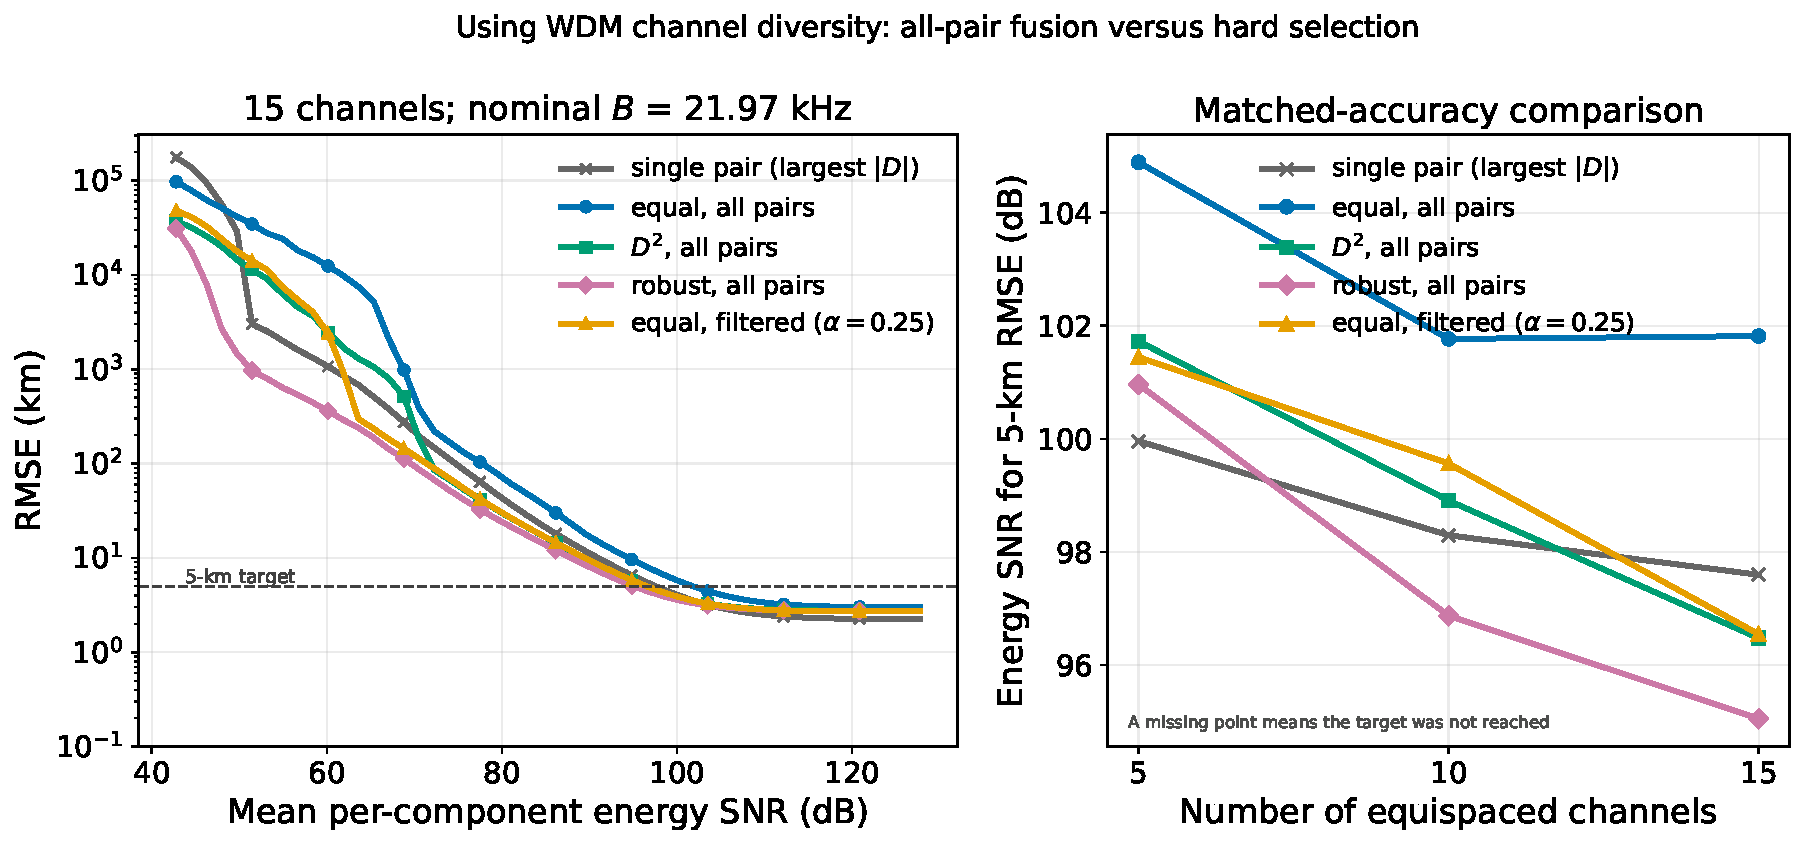
\includegraphics[width=0.90\linewidth]{F10_equispaced_fusion_strategy_vector.pdf}
\caption{EQUISPACED GRID: empirical distance RMSE and energy SNR needed for a 5-km localization error as channel count increases.}
\label{fig:fusion}
\end{figure}

Figure~\ref{fig:weights} explains the equispaced-grid result. Fifteen channels produce 105 pairs with a graded spread of CD sensitivities, rather than a clean split into good and bad pairs. At $\alpha=0.25$, the hard filter keeps the 32 pairs with $|D_{ij}|\ge0.5D_{\max}$ and discards the other 73. Under all-pair $D^2$ weighting, each pair receives a normalized share proportional to $D_{ij}^2$; those 73 lower-sensitivity pairs still carry 26.2\% of the total assigned weight. Thus continuous weighting retains a material contribution from pairs that the hard cutoff deletes. By contrast, on the 12-channel alternating band-edge grid, dispersion separates into low- and high-sensitivity groups: the filter keeps 36 of 66 pairs, and the excluded pairs carry only 0.011\% of total $D^2$ weight. At $B_{\rm nom}=22.51$\,kHz, the 5-km target requires 119.84\,dB for equal all-pair averaging, versus 90.02\,dB for all-pair $D^2$ or robust fusion and 90.01\,dB for filtered equal averaging. Figure~\ref{fig:bandedge-snr} highlights this 29.8-dB reduction. These weight shares describe the fusion rule's allocation, not independent statistical information.

\begin{figure}[tb]
\centering
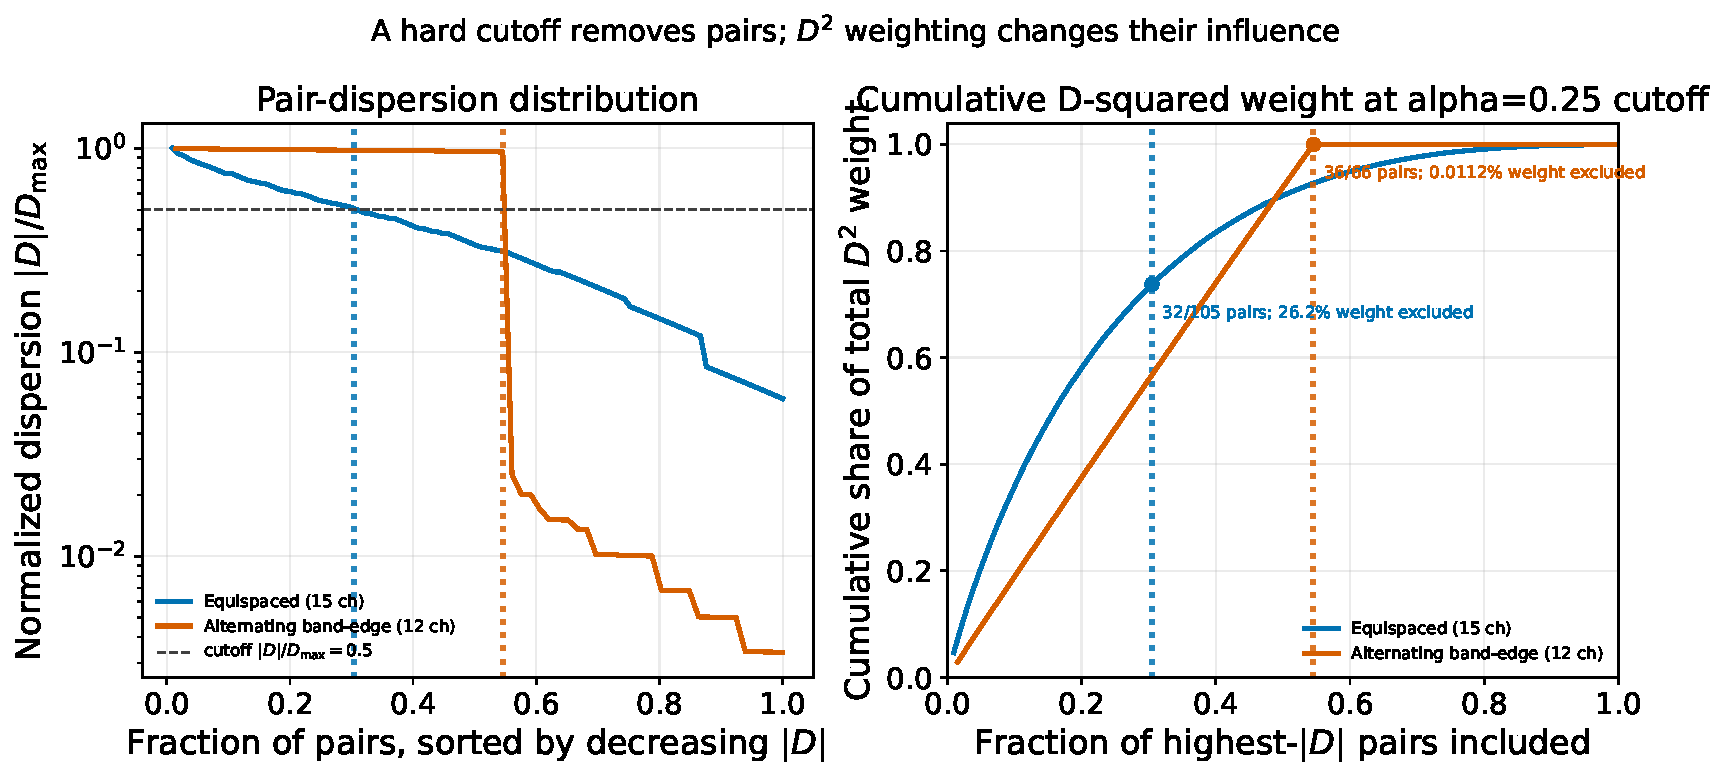
\includegraphics[width=0.80\linewidth]{F11_pair_weight_distribution_vector.pdf}
\caption{Pair-dispersion distributions and cumulative $D^2$ weight. A graded equispaced grid retains appreciable weight below the hard cutoff; the band-edge layout nearly separates useful and weak pairs.}
\label{fig:weights}
\end{figure}

\begin{figure}[tb]
\centering
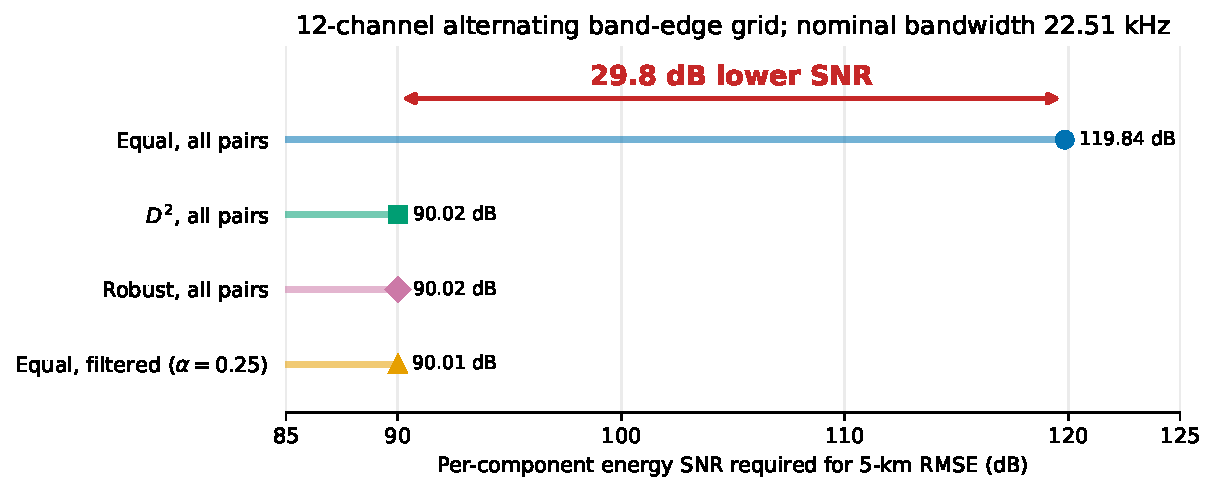
\includegraphics[width=0.74\linewidth]{bandedge_target_snr_vector.pdf}
\caption{Per-component energy SNR required for 5-km distance RMSE on a 12-channel alternating band-edge grid at $B_{\rm nom}=22.51$\,kHz. Dispersion-aware fusion saves 29.8\,dB relative to equal all-pair averaging.}
\label{fig:bandedge-snr}
\end{figure}

\section{Estimator choice, implications, and limits}
Delay-estimator choice is regime-dependent. Near $22$\,kHz and 127.8\,dB, robust fusion gave 2.64\,km distance RMSE with parabolic interpolation and 0.71\,km with generalized cross-correlation with phase transform (GCC-PHAT) \cite{knapp1976}; near $1.3$\,kHz and 103.8\,dB, parabolic was better (25.8 versus 52.3\,km). Parabolic interpolation often has lower variance but a bias floor; GCC-PHAT can reduce bias, although weak spectral bins can mislead it. We therefore compare distance RMSE, not variance alone.

At high SNR, spread approximately scales as $\sigma_Z\propto(\sqrt{\SNR_E}B_{\rm nom})^{-1}$; more channels often reduce the required SNR, while averaging independent fibres reduces spread roughly as $N_{\rm fib}^{-1/2}$. A practical design sequence is to check cross-channel observability, inspect pair dispersion, compare equal, $D^2$, and robust fusion, then choose the delay estimator using both bias and spread. Since pairs reuse channel records, their errors can be correlated; the $N(N-1)/2$ pair estimates are not independent.

These results establish a practical design principle for WDM transient localization: channel diversity is most useful when pair dispersion guides fusion. On the band-edge grid, dispersion-aware fusion saves 29.8\,dB for the 5-km target; robust fusion also improves the equispaced case. The method can localize mechanical, lightning-associated, or other events when they produce a detectable shared SOP signature. The present evidence is from a localized simulation and motivates field validation.

\begin{multicols}{2}
\begin{thebibliography}{13}\scriptsize
\setlength{\itemsep}{0pt}\setlength{\parskip}{0pt}
\bibitem{mecozzi2021} A. Mecozzi, M. Cantono, J. C. Castellanos, V. Kamalov, R. Muller, and Z. Zhan, ``Polarization sensing using submarine optical cables,'' \emph{Optica} \textbf{8}(6), 788--795 (2021). doi:10.1364/OPTICA.424307.
\bibitem{mecozzi2025} A. Mecozzi et al., ``Geophysical sensing using Jones matrices extracted from submarine optical cable transceivers carrying live traffic,'' \emph{Optica} \textbf{12}(11), 1712--1719 (2025). doi:10.1364/OPTICA.572883.
\bibitem{vaskinn2025} K. S. Vaskinn et al., ``Localising state-of-polarisation perturbation on a repeatered link using wavelength dispersion delay walk-off,'' in \emph{Optical Fiber Communication Conference}, Th2A--39 (2025). doi:10.1364/OFC.2025.Th2A.39.
\bibitem{tang2024} J. Tang et al., ``Forward-transmission based distributed fiber sensing compatible with C+L unidirectional communication systems,'' in \emph{2024 Optical Fiber Communications Conference and Exhibition (OFC)}, 1--3 (2024). doi:10.1364/OFC.2024.W2A.12.
\bibitem{gordon2000} J. P. Gordon and H. Kogelnik, ``PMD fundamentals: Polarization mode dispersion in optical fibers,'' \emph{Proc. Natl. Acad. Sci. USA} \textbf{97}(9), 4541--4550 (2000). doi:10.1073/pnas.97.9.4541.
\bibitem{shtaif2005} M. Shtaif and A. Mecozzi, ``Modelling of polarization mode dispersion in optical communications systems,'' in \emph{Polarization Mode Dispersion}, A. Galtarossa and C. R. Menyuk, Eds. (Springer, 2005), pp. 34--51. doi:10.1007/0-387-26307-1\_2.
\bibitem{gisin1992} N. Gisin and J. P. Pellaux, ``Polarization mode dispersion: time versus frequency domains,'' \emph{Opt. Commun.} \textbf{89}(2--4), 316--323 (1992).
\bibitem{corning2020} Corning Incorporated, ``Corning Vascade optical fibers product information,'' Product Information Sheet PI1445 (Mar. 2020). Available: \url{https://www.corning.com/media/worldwide/coc/documents/Fiber/product-information-sheets/PI-1445-AEN.pdf}.
\bibitem{corning2023} Corning Incorporated, ``Corning Vascade EX2000 optical fiber product information,'' Product Information Sheet PI1440 (Mar. 2023). Available: \url{https://www.corning.com/media/worldwide/coc/documents/Fiber/product-information-sheets/PI-1440.pdf}.
\bibitem{weiss1983} A. J. Weiss and E. Weinstein, ``Fundamental limitations in passive time-delay estimation---Part I: Narrowband systems,'' \emph{IEEE Trans. Acoust., Speech, Signal Process.} \textbf{31}(2), 472--485 (1983).
\bibitem{sadler2006survey} B. M. Sadler and R. J. Kozick, ``A survey of time delay estimation performance bounds,'' in \emph{Proc. Fourth IEEE Workshop on Sensor Array and Multichannel Processing}, 282--288 (2006).
\bibitem{knapp1976} C. Knapp and G. Carter, ``The generalized correlation method for estimation of time delay,'' \emph{IEEE Trans. Acoust., Speech, Signal Process.} \textbf{24}(4), 320--327 (1976).
\end{thebibliography}
\end{multicols}

\end{document}
